\chapter{Configuración del Vocabulario} \label{cap:05Vocab}

El vocabulario no viene enteramente configurado en ATLAS Broadsea sino tan solo una pequeña demo adjunta a la base de datos de Eunomia (véase \ref{01.4Postgre}).

Por tanto, para utilizar ATLAS se requiere la instalación y configuración del Vocabulario más extenso. OHDSI propone, en el repositorio de github de Broadsea \ref{cap:05Vocab} dos formas de configurar el vocabulario de Broadsea: (1) de forma manual (2) a través de Apache Solr. 

\section{Configuración manual}

La configuración manual del vocabulario requiere descargar el vocabulario directamente desde ATHENA \cite{athena}, instalarlo manualmente en el directorio local de Broadsea y ejecutar el contenedor docker encargado de montar el vocabulario en Broadsea. 

\subsection{Requisitos previos}

Para configurar el vocabulario manualmente,  se debe haber descargado el vocabulario y configurado el directorio local de Broadsea. Este procedimiento se ha seguido gracias a los foros ''Downloading OMOP cdm version 5 vocabulary data'' \cite{forumCDMdownload} y ''March to the Broadsea'' \cite{forumMarchBroadsea} y el tutorial de yotutube ''Demo: Getting Vocabularies Into My OMOP CDM'' \cite{youtubeVocab}

\begin{enumerate}

    \item Descargar el vocabulario desde la herramienta online de  ATHENA.Para ello, acceder al menú de descarga \code{Download}. En este momento se presenta un listado de todos los vocabularios que contiene ATHENA entre los que algunos aparecen preseleccionados. Cada usuario puede seleccionar o deseleccionar los vocabularios que le interesen para el estudio que esté realizando. En este caso, se descargará el vocabulario que ATHENA sugiere por defecto.
    
    \begin{figure}[H]
        \centering
        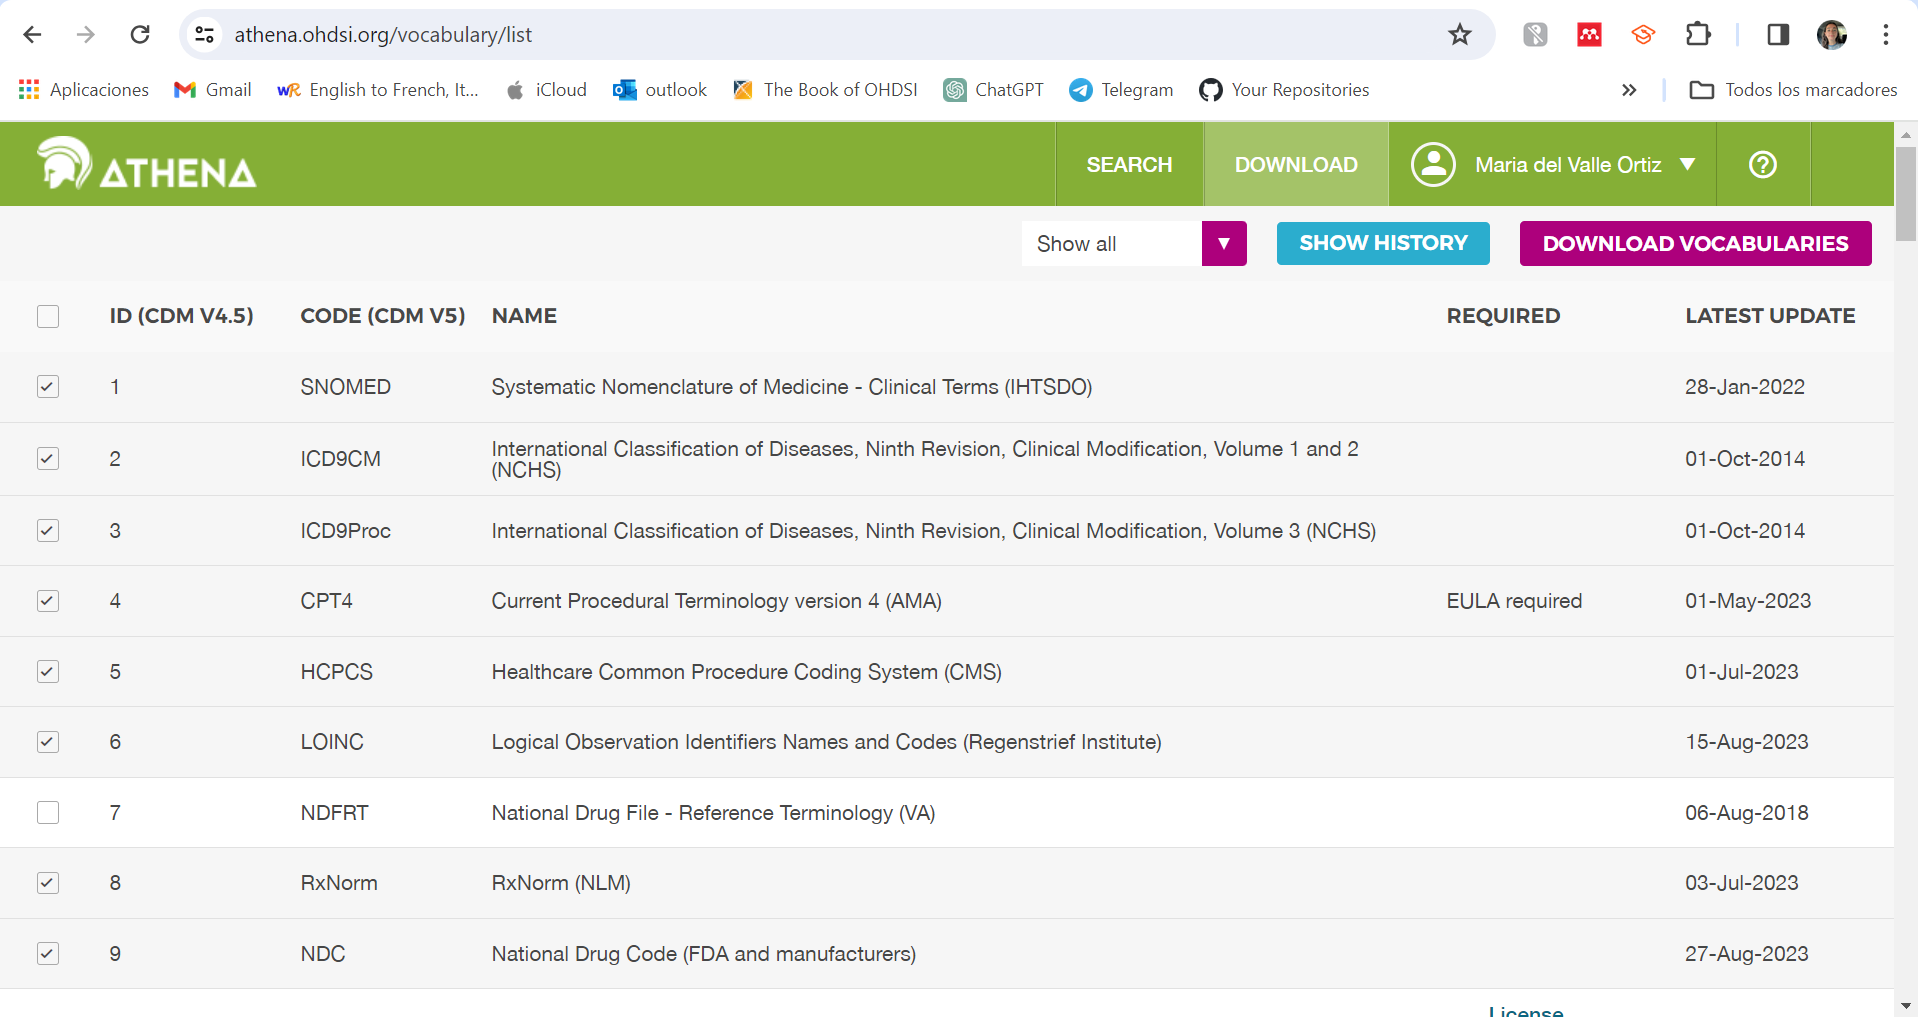
\includegraphics[width=0.90\textwidth]{figures/athenaPreDownload.png}
        \caption{Captura de pantalla de la preselección de vocabularios para descargar.}
        \label{fig:athenaPreDownload}
    \end{figure}

    \item La descarga requiere registrar un usuario con un correo electrónico válido al que se enviará un link personal que permitirá la descarga de un archivo .zip con el vocabulario seleccionado. También desde ATHENA en la pestaña \code{SHOW HISTORY} muestra el estado en el que se encuentra la descarga del vocabulario y, una vez que esté listo, permite la descarga directa del zip.

    \item El archivo zip que se descarga, una vez descomprimido, muestra varios archivos .csv con las tablas que conforman el Vocabulario y otros archivos CPT4 que requieren de una configuración adicional. En este caso, no se utilizará el vocabulario de CPT4 por lo que no se realizará esta configuración, sin embargo, viene bien explicada en el tutorial de youtube adjunto al principio de la sección.

      \begin{figure}[H]
        \centering
        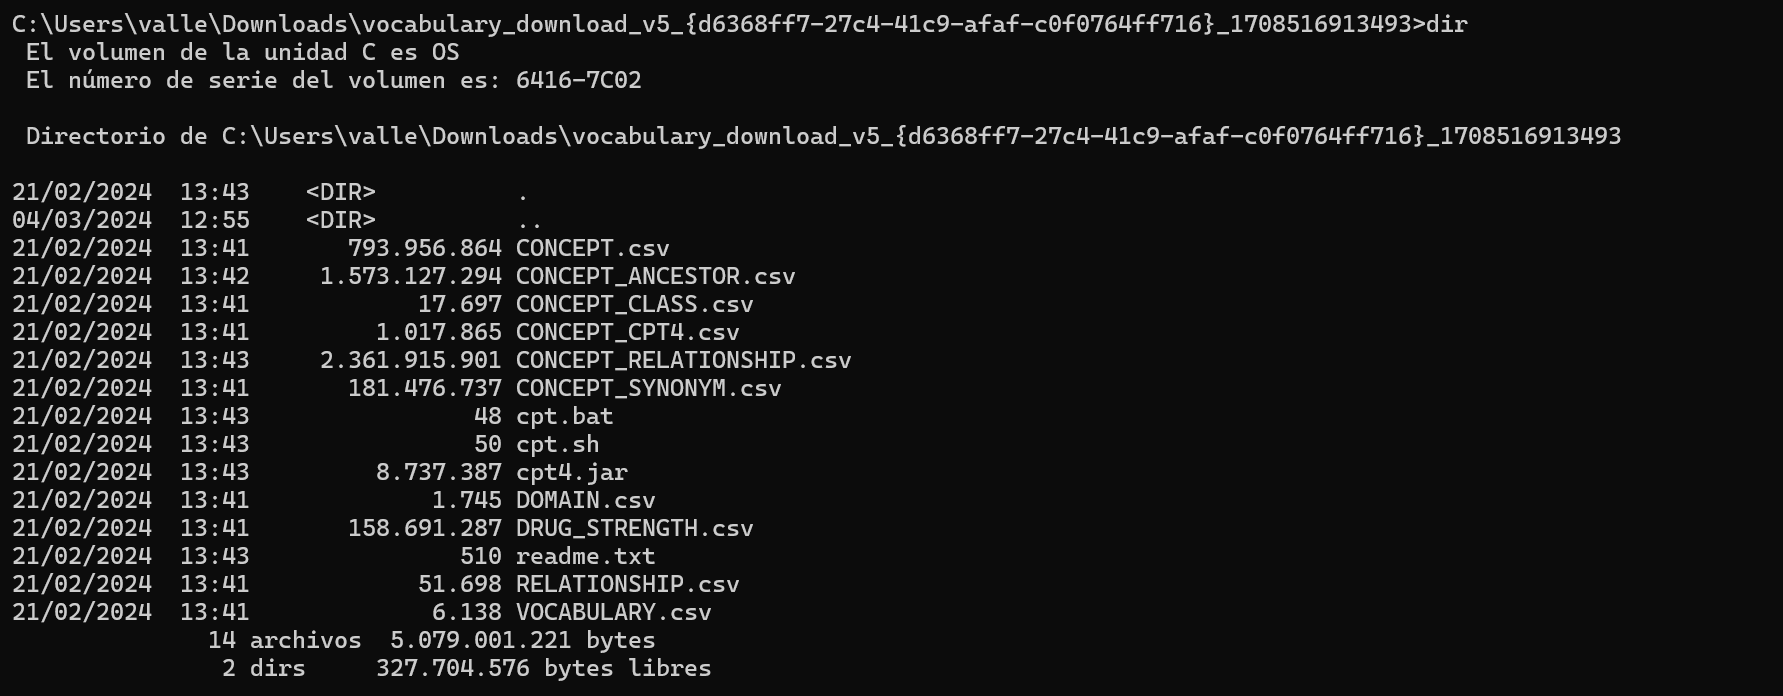
\includegraphics[width=0.90\textwidth]{figures/vocabDownload.png}
        \caption{Captura de pantalla de archivos descargados del vocabulario.}
        \label{fig:vocabDownload}
    \end{figure}

    \item Por último, los archivos descargados del vocabulario deben almacenarse en el directorio local de Broadsea, concretamente en la ruta \code{Broadsea/omop\_vocab/files}. En caso de no existir la carpeta \code{/files}, crearla manualmente. Este paso es muy importante.

\end{enumerate}

\subsection{Deployment}

Configurar el vocabulario requiere establecer una configuración avanzada del contenedor Docker de Broadsea. Si bien, la primera vez que se inicializó el contenedor se ejecutó el perfil \code{default} ahora se va a ejecutar específicamente el perfil \code{omop-vocab-pg-load}. Esta opción se especifica en la sección \code{OMOP Vocab Loading} del repositorio de Broadsea. También ha sido de utilidad el repositorio \cite{githubCDMConfig} y el mismo foro \cite{forumMarchBroadsea}.

Para acceder a la información y configuración avanzada del perfil se puede acceder al \code{docker-compose.yml} y a la sección 9 del archivo \code{.env}, aunque este caso no será necesario realizar ninguna modificación sobre los mismos.

\begin{enumerate}

    \item Para comenzar la configuración del vocabulario es necesario inicializar el contenedor \code{omop-vocab-load}. Ejecutar la siguiente línea de código en el \code{cmd}:

    \begin{lstlisting}[language=sh]
    docker compose --profile omop-vocab-pg-load up -d\end{lstlisting}

    Este comando da lugar el siguiente resultado.

      \begin{figure}[H]
        \centering
        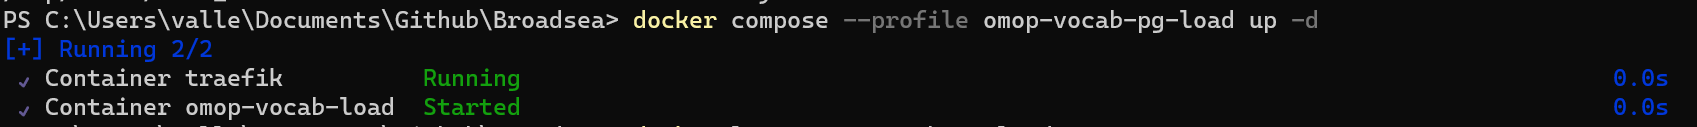
\includegraphics[width=0.90\textwidth]{figures/composeProfVocabLoad.png}
        \caption{Captura de pantalla de comando para iniciar el perfil docker.}
        \label{fig:composeProfVocabLoad}
    \end{figure}

    \item A partir de este momento comienza la instalación del perfil, por lo que es muy importante tener abierto el \code{logs} de Docker para poder observar que el proceso se realiza correctamente. El proceso puede durar unas horas y una vez que se finaliza, el log muestra un mensaje que advierte que el contenedor puede ser eliminado y el estado del contenedor pasa a ser ''Exited''. El resultado es la creación de un nuevo esquema en la base de datos llamado ''omop\_vocab'' con todos los archivos descargados del vocabulario. 

    \item El último paso de la configuración es integrar este nuevo esquema a la WebAPI de Broadsea. Este último paso se puede realizar fácilmente de forma manual a través de pgAdmin, abriendo la tabla \code{source\_daimon} del esquema \code{webapi} de la bd de Broadsea.

    La instalación por defecto de Broadsea adjudica la fuente del vocabulario (\code{daimon\_type=1}) al \code{demo\_cdm}, sin embargo, se debe modificar para que apunte al nuevo esquema \code{omop\_vocab} que se ha instalado. Esta modificación se puede realizar directamente haciendo click ssobre la tabla que devuelve la siguiente consulta.

    \begin{lstlisting}[language=sql]
    SELECT * FROM webapi.source_daimon
    ORDER BY source_daimon_id ASC \end{lstlisting}

    El resultado final debe ser similar a la siguiente figura.

    \begin{figure}[H]
        \centering
        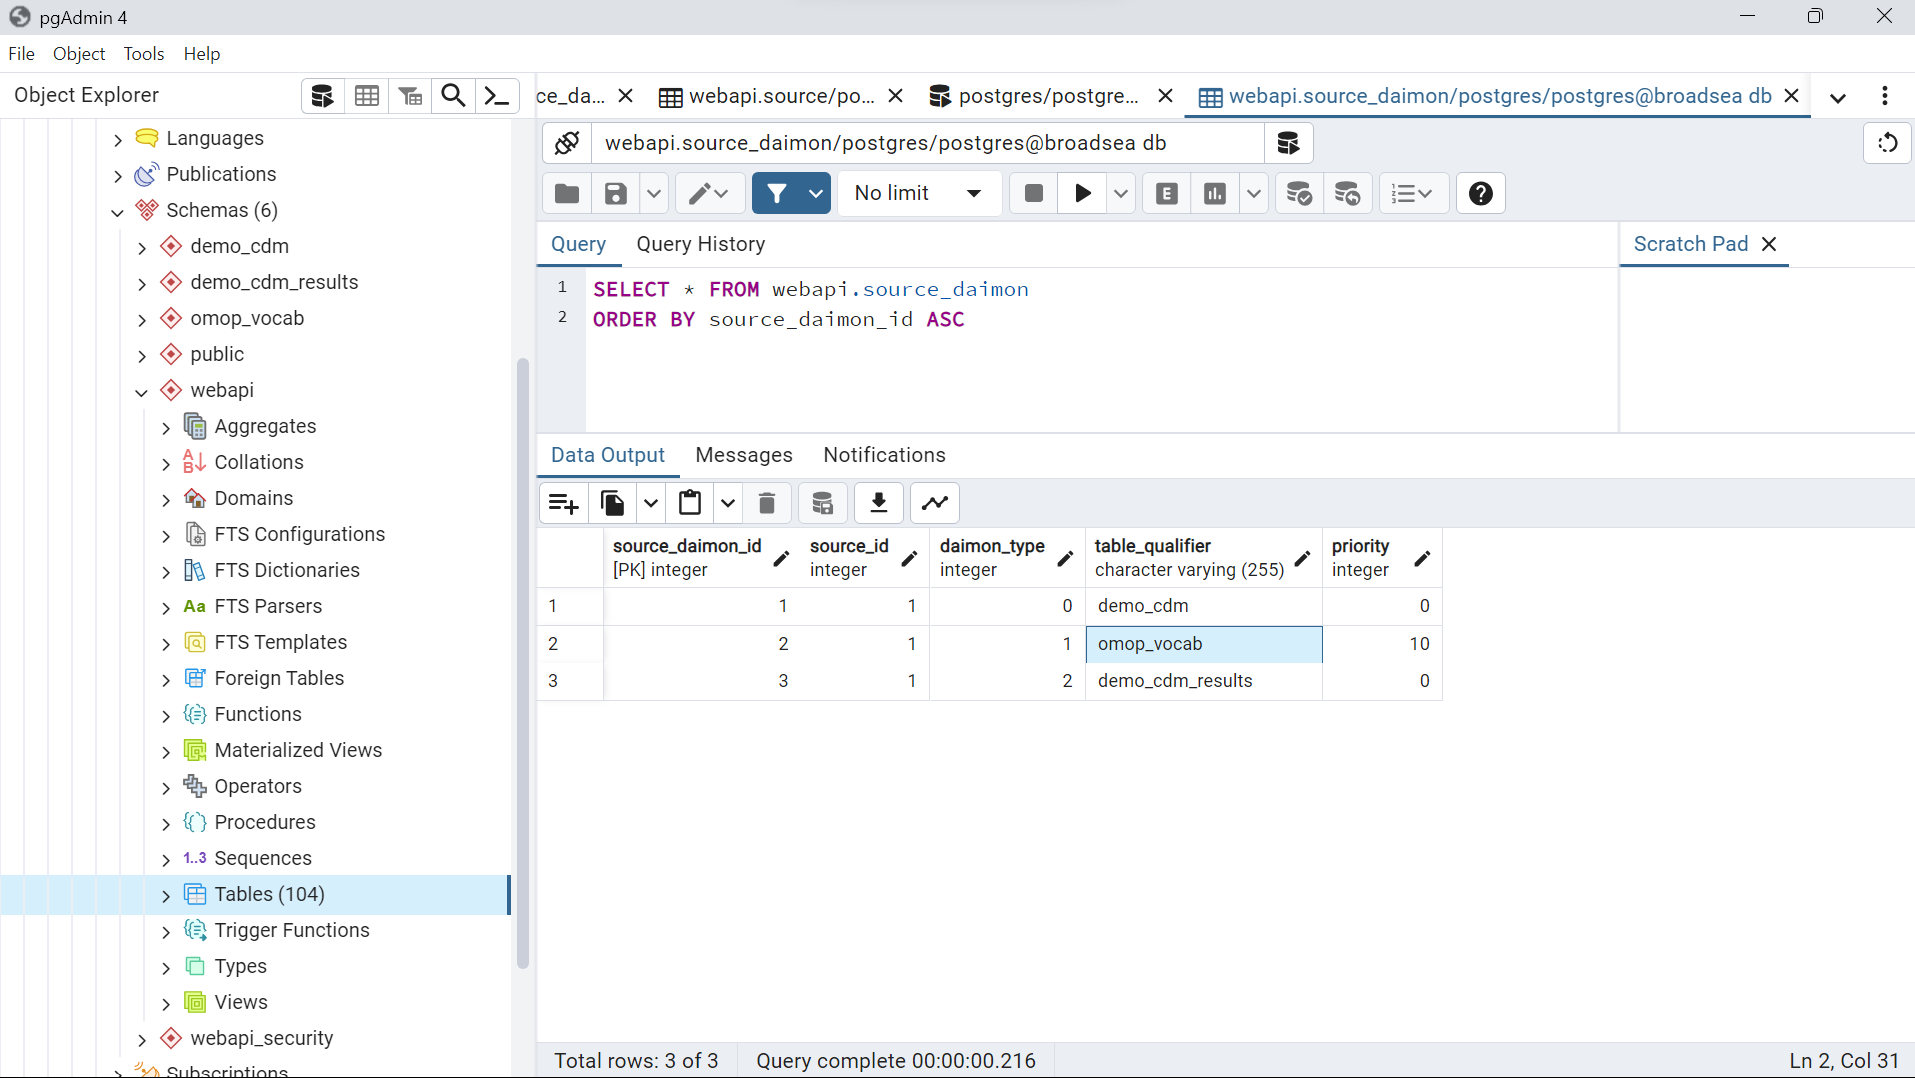
\includegraphics[width=0.90\textwidth]{figures/omopVocabResult.png}
        \caption{Captura de pantalla de la integración final del vocabulario descargado con la webapi}
        \label{fig:omopVocabResult}
    \end{figure}

\end{enumerate}

\subsection{Comprobación de configuración correcta}

Para comprobar que se ha configurado correctamente el vocabulario en la base de datos de Broadsea, se puede consultar el administrador de la base de datos o realizar directamente una búsqueda en ATLAS.

\begin{enumerate}

    \item En primer lugar, desde el administrador de la base de datos, pgAdmin, se debe comprobar que el vocabulario se ha instalado correctamente y no se han instalado tablas vacías. Para ello basta con seleccionar cualquier tabla del esquema \code{omop\_vocab} y mostrar todas las filas. Las tablas más significativas son la tabla \code{vocabulary}, que muestra todos los vocabularios que se han insertado, y la tabla \code{concept} que reúne todos los conceptos definidos en cada vocabulario. Para esta implementación la primera tabla muestra un total de 59 filas y la segunda, 5.975.392 filas.

    \item En segundo lugar, se puede comprobar que la integración del nuevo esquema con el vocabulario haya sido exitosa realizando una búsqueda en el vocabulario directamente desde ATLAS Broadsea. 
    
    El vocabulario demo que venía incluido con Eunomia presentaba muy pocos conceptos por lo que muchas búsquedas de conceptos no devolvían resultado o devolvían muy pocos. Para este manual, se comprobó que antes de realizar la configuración del vocabulario, al buscar ''diabetes'' solo se obtenía un resultado, como se muestra en la figura \ref{fig:ejDiabetesVacio}. Sin embargo, después de configurar correctamente, se obtienen hasta 20602 resultados, como muestra la figura \ref{fig:ejDiabetsFull}.

        \begin{figure}[H]
        \centering
        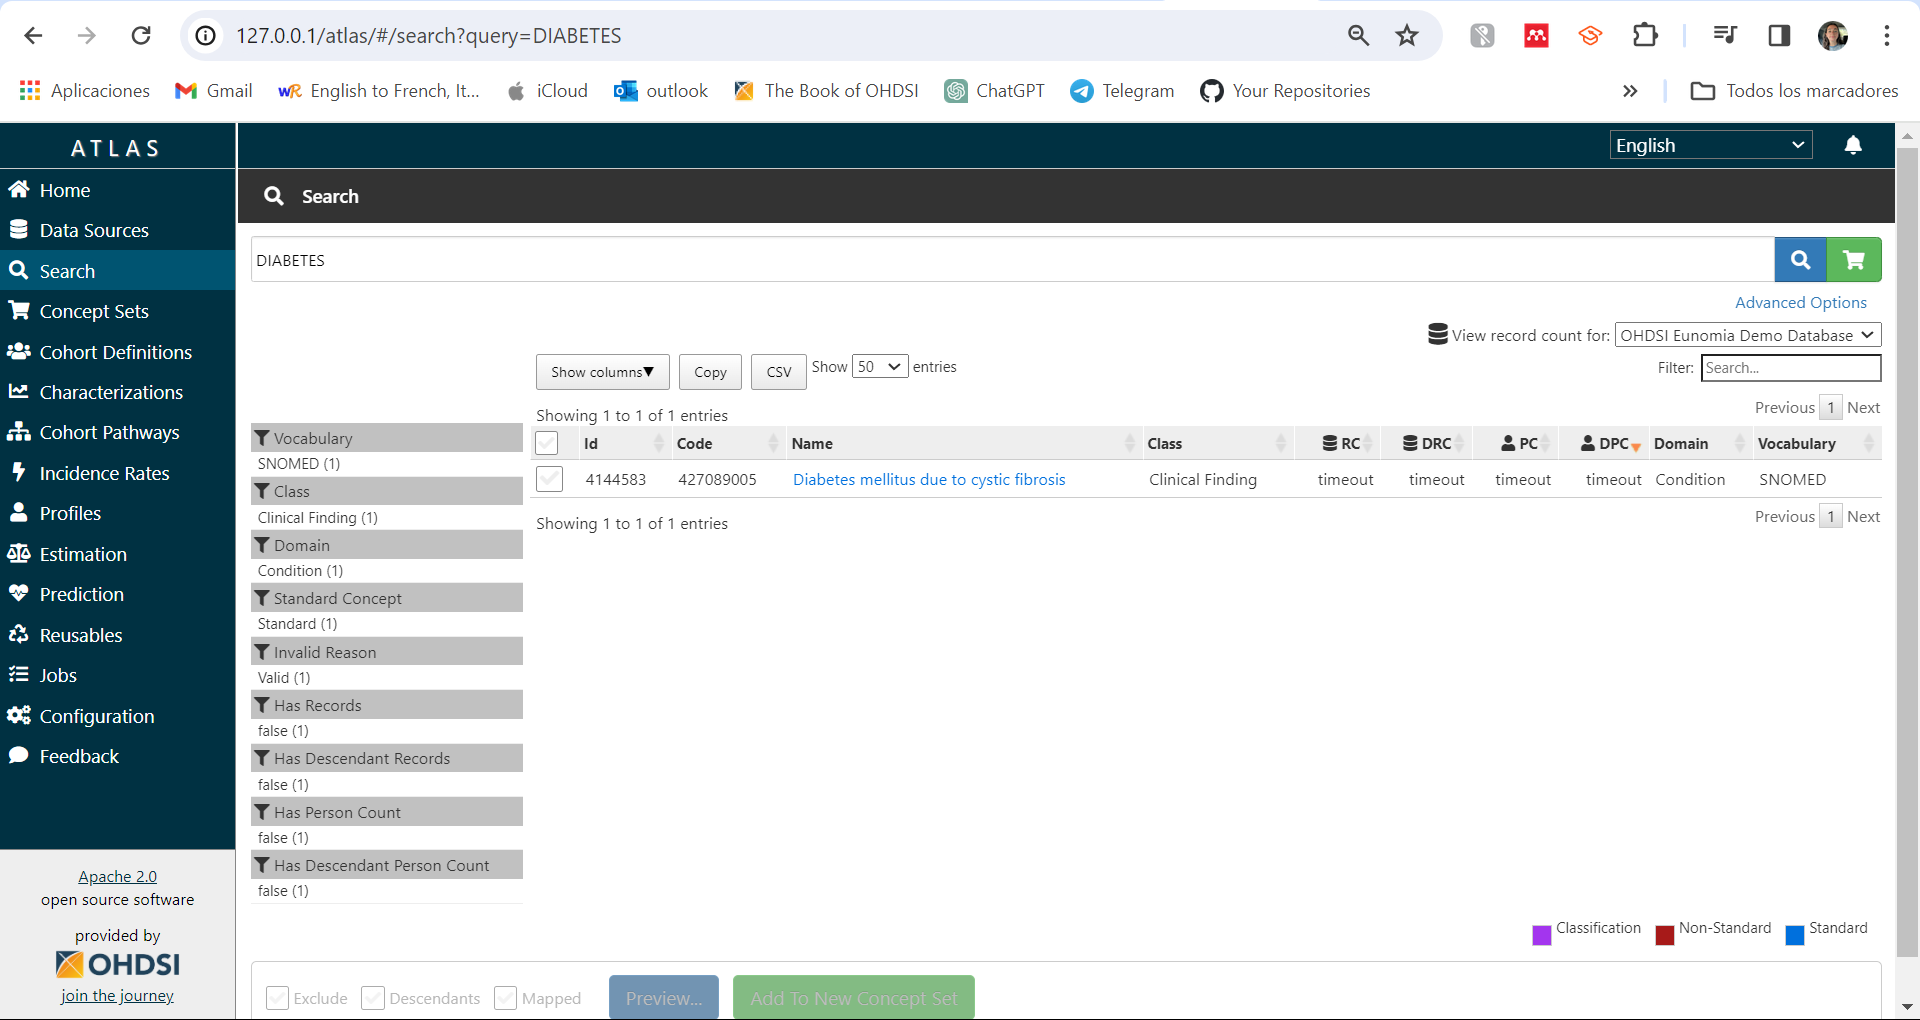
\includegraphics[width=0.90\textwidth]{figures/ejDiabetesVacio.png}
        \caption{Captura de pantalla de la búsqueda en el vocabulario antes de la configuración}
        \label{fig:ejDiabetesVacio}
    \end{figure}

      \begin{figure}[H]
        \centering
        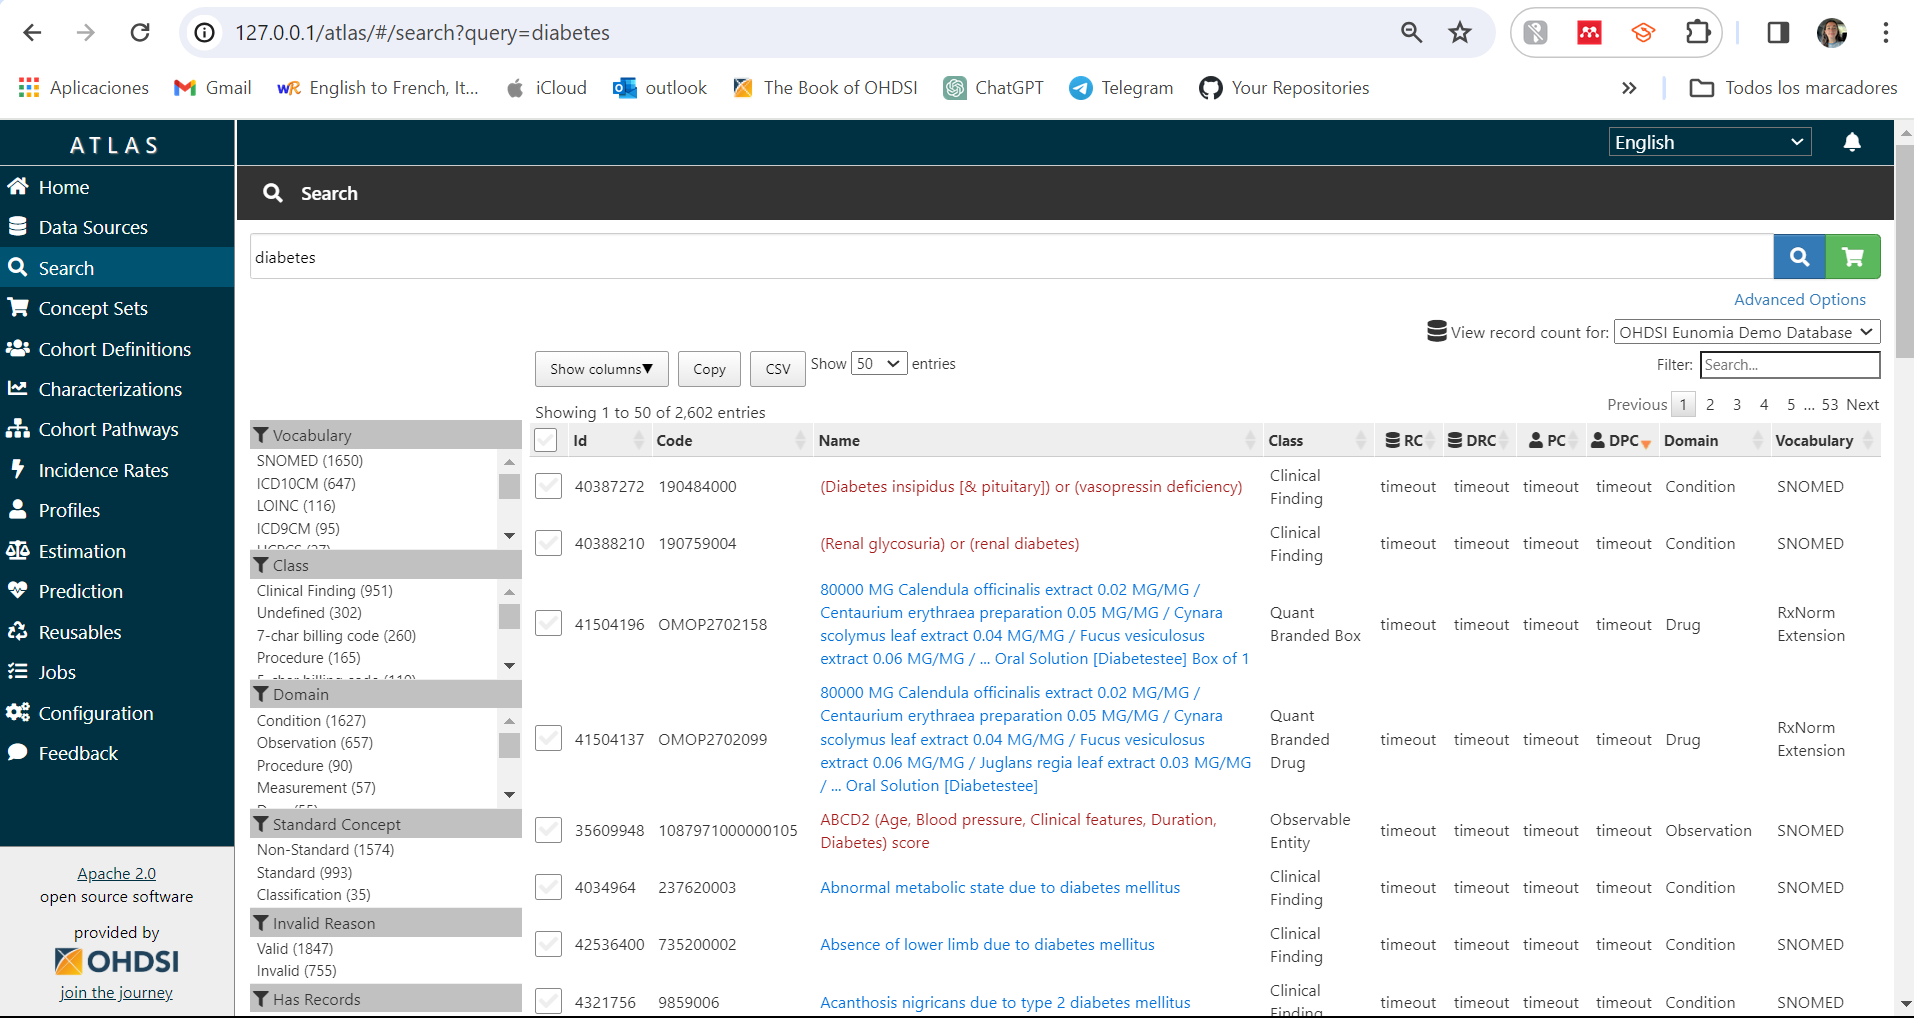
\includegraphics[width=0.90\textwidth]{figures/ejDiabetsFull.png}
        \caption{Captura de pantalla de la búsqueda en el vocabulario después de la configuración}
        \label{fig:ejDiabetsFull}
    \end{figure}

    \item Por último, se puede realizar una comprobación extra accediendo a la dirección \code{http://127.0.0.1/WebAPI/source/refresh} en el navegador, que imprime en pantalla las fuentes que se están utilizando en la configuración de Broadsea. El resultado debe ser similar al siguiente, prestando especial atención a que aparezca \code{omop\_vocab} como fuente del vocabulario:


    \begin{lstlisting}[language=html]
    [{"sourceId":1,"sourceName":"OHDSI Eunomia Demo Database","sourceDialect":"postgresql","sourceKey":"EUNOMIA","daimons":[{"sourceDaimonId":1,"daimonType":"CDM","tableQualifier":"demo_cdm","priority":0},{"sourceDaimonId":3,"daimonType":"Results","tableQualifier":"demo_cdm_results","priority":0},{"sourceDaimonId":2,"daimonType":"Vocabulary","tableQualifier":"omop_vocab","priority":10}]}] \end{lstlisting}

    
\end{enumerate}


\subsection{Solución de posibles errores}

\subsubsection{Error: can't cd to /temp/files: No such files or directory}

Al inicializar el perfil \code{omop-vocab-load} el contenedor no se construye correctamente y el log muestra el siguiente aviso, tal y como se muestra en la figura.

      \begin{figure}[H]
        \centering
        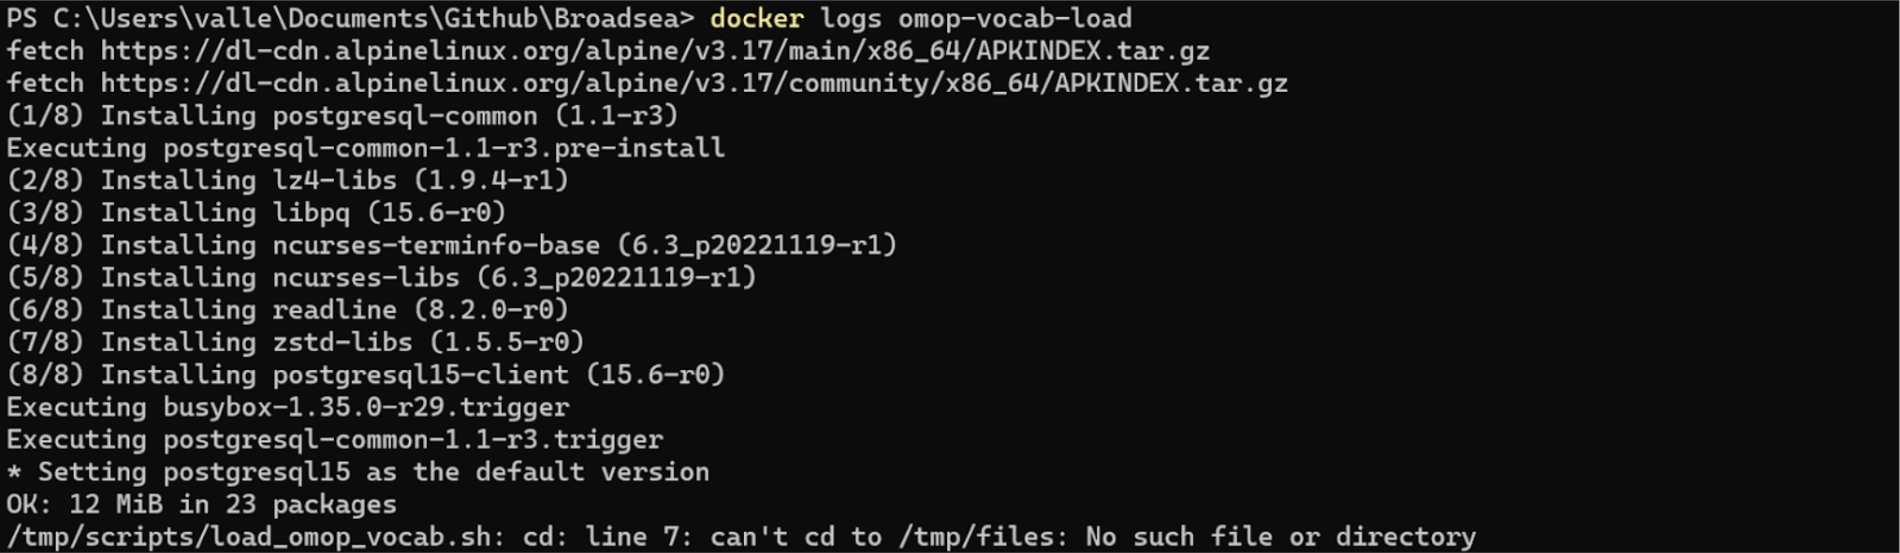
\includegraphics[width=0.90\textwidth]{figures/error05NoFile.png}
        \caption{Captura de pantalla de la búsqueda en el vocabulario después de la configuración}
        \label{fig:error05NoFile}
    \end{figure}
    
Solución: Crear manualmente la carpeta /files

\subsubsection{Error: El contenedor se construye correctamente pero se construye vacío}

Al inicializar el perfil \code{omop-vocab-load} el contenedor se construye en pocos segundos aparentemente correctamente. Incluso es posible que aparezca en el administrador de la base de datos pero aparece el esquema vacío o las tablas del esquema vacías, sin filas.

Solución: La carpeta /files debe contener los archivos .csv que se han descargado de ATHENA.

\section{Otras configuraciones avanzadas}

En este punto el vocabulario ya está perfectamente instalado y configurado, sin embargo, Broadsea ofrece más opciones avanzadas para sacar aún mayor partido de la herramienta. En este manual se presentan dichas opciones aunque no se procederá a su configuración.

\subsection{Configuración de Apache Solr}

ATLAS Broadsea hace uso de Apache Solr a través de diferentes perfiles docker para facilitar la importación del vocabulario y la búsqueda en el mismo. Sin embargo, ambas características aún se encuentras en desarrollo, según la información facilitada en el repositorio de github de Broadsea Solr \cite{githubBroadseaSolr}.

El proceso de configuración de Broadsea Solr se encuentra en aquel mismo repositorio y la descripción de los perfiles que ejecutan los contenedores Solr se presentan en el de Broadsea \cite{githubBroadsea}. 

\begin{enumerate}
    \item Con el perfil \code{solr-vocab-with-import} se puede automatizar la importación del vocabulario desde el servidor de Apache en vez de tener que configurarlo manualmente. Sin embargo, esta opción que parece facilitar el trabajo al usuario en la práctica resulta engorrosa, por ello no ha sido cubierta en este manual.
    \item El otro perfil, \code{solr-vocab-no-import} simplemente lanza el servidor Apache ''vacío'' permitiendo la configuración manual del vocabulario desde la GUI de Apache Solr.
\end{enumerate}

Para mayor información o resolución de conflictos consultar los foros de OHDSI o los ''issue'' del repositorio de github.

\subsection{Configuración de PHOEBE}

ATLAS Broadsea puede configurarse junto a PHOEBE, que es una herramienta OHDSI, también disponible \href{https://data.ohdsi.org/PHOEBE/}{online}, que consiste en un recomendador de conceptos del vocabulario, de forma que facilite la construcción de conjuntos de conceptos durante la realización de estudios con ATLAS. 

No existe un repositorio concreto de esta herramienta pero el perfil que implementa el contenedor docker se presenta brevemente en el repositorio de \href{https://github.com/OHDSI/Broadsea}{Broadsea}. También se puede encontrar información relevante en algunos foros de OHDSI como en el de \href{https://forums.ohdsi.org/t/phoebe-2-0/17410}{Phoebe 2.0}.

De igual forma, para mayor información o resolución de conflictos consultar otros foros de OHDSI o los ''issue'' del repositorio de github de Broadsea o ATLAS.